\section{Methods}

\begin{figure}[h]
    \centering
    \includegraphics[width=\linewidth]{figures/mini_pipeline.pdf}
    \caption{
        \textbf{The MINI pipeline.} \\
        \small The MINI pipeline is comprised of 4 steps: 1) Spatiotemporal binning and processing of neural data; 2) Model training; 3) Model evaluation (and optional re-training); 4) Latent evaluation for feature interpretability. Steps 1-3 including model re-training, can be either semi- or fully-automated.
    }
    \label{fig:mini_pipeline}
\end{figure}

\begin{figure}[h]
    \begin{minipage}{0.64\linewidth}
    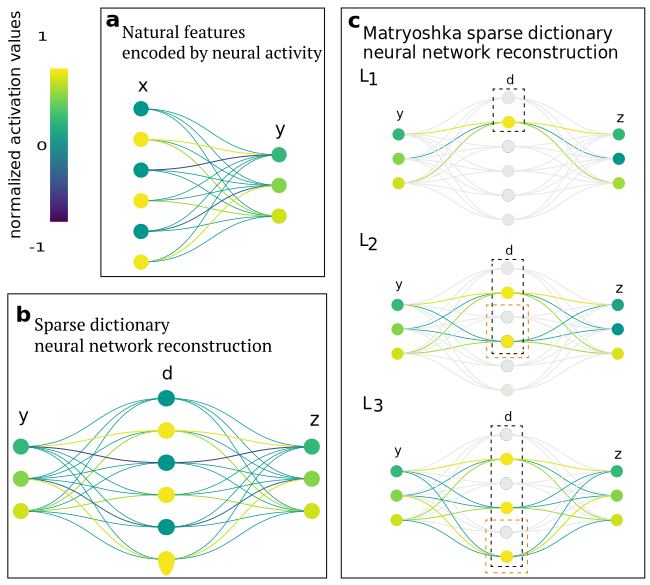
\includegraphics[width=\linewidth]{figures/sdnn_arch.pdf}
    \end{minipage}%
    \begin{minipage}{0.35\linewidth}
    \caption{
        \textbf{Model motivation} \\
        \small
        (\textbf{a}) Natural ("real-world") features $x$ get encoded by neural activity $y$. At this timepoint, three active features are simultaneously represented by the joint activity of three neurons. (\textbf{b}) A neural network reconstructs neural activity $z$ from $y$ via sparse dictionary elements $d$. When training is successful, $d$ corresponds to $x$: sparse dictionary elements represent natural features. If $z$ tries to recreate $y$ exactly ($\hat{y}$), the model is an autoencoder; in other scenarios (e.g. $\z$ is separate but dependent on or related to $y$) it is a transcoder or crosscoder. (\textbf{c}) A Matryoshka spare dictionary neural network segments the latent space into multiple levels, each of which attempts to do a full reconstruction of the target neural activity. In this case, latents exclusive to the highest-level will often correspond to high-level features (e.g. a round object), while latents exclusive to the lowest-level will often correspond to low-level features (e.g. a basketball).
    }
    \label{fig:sdnn_arch}
    \end{minipage}
\end{figure}

MINI takes in high-dimensional neural data and outputs interpretable features of this data. The semi-automated pipeline consists of four steps (\autoref{fig:mini_pipeline}), the first three of which can be fully automated.

In step 1, data processing is performed to prepare the neural data for model training. MINI contains code to take the output from common spikesorters (e.g. kilosort ~\cite{pachitariu_2016_kilosort}), bin it into a 2D matrix of time X space (e.g. timebins, units (putative neurons)), and normalize the data (e.g. max normalize or z-score normalize across space (e.g. units) or time (e.g. timebins)). Users can also manually bin and process their data before proceeding to step 2.

In step 2, a SDNN is trained on the processed neural data. This step includes hyperparameter optimization, which can be done via grid search or other methods. Variant of MSAE as SAE. Transformer decoder layer. Show latex formulas for encoder, decoder, total loss.

In step 3, the trained model is evaluated using a variety of metrics to assess its performance. If the model does not meet the desired criteria, it can be re-trained with different hyperparameters. 

Finally, in step 4, the latents produced by the model are evaluated for interpretability as features. This includes visualizing their activation patterns over time and experimental conditions, as well as assessing their decoding performance. The user can then export these features for further analysis.

Example usage of the pipeline on multiple distinct datasets can be found in notebooks mentioned in \nameref{subsection:software_data_availability}.

- For a user, the full, semi-automated pipeline is as follows:
\begin{enumerate}
    \item Data processing
    \begin{itemize}
        \item Spatiotemporally bin and normalize
        \begin{itemize}
            \item MINI has a convenience function to do this directly from output of common spikesorters (kilosort), where we bin unit spikes given a specified timebin and optionally normalize (z-score or max) dataset across time and/or unit
            \begin{itemize}
                \item (and similar approach could be applied to output from common calcium imaging processing (e.g. Suite2p))
            \end{itemize}
        \end{itemize}
    \end{itemize}
    
    \item Model training
    \begin{itemize}
        \item Hyperparameter optimization
        \begin{itemize}
            \item Model parameters
            \item Optimizer parameters
        \end{itemize}
        \item By default no validation set, but can be added if we want to e.g. apply to other recordings of same animal, though this is not generally recommended (just train a freshie)
    \end{itemize}
    
    \item Model evaluation
    \begin{itemize}
        \item (We implement all metrics from SAEBench which are not language-model specific, plus a couple of our own)
        \item L0 of latents
        \item R\textsuperscript{2} (var explained) and cos sim of reconstruction-to-actual neural activity for each spatial bin, and each temporal bin
        \item Latent density histogram (as in SAEBench)
        \item Variance explained of overall reconstruction from each latent (variance shouldn't be in just a few features) ?
        \item Spectral frequency analysis to ensure temporal frequency content is preserved?
    \end{itemize}
    
    \item Feature evaluation
    \begin{itemize}
        \item When a latent is subjectively determined to be sufficiently interpretable, we call this a feature.
        \item Interactive plots showing feature activation patterns across time and experimental conditions.
        \item We evaluate its decoding performance?
        \item Export functionality.
    \end{itemize}
\end{enumerate}

For additional detail on the pipeline, see \nameref{subsection:additional_pipeline_details}.

For additional detail on model architecture, see \nameref{subsection:additional_model_details}.

\subsection{Neural Data Pipeline}

\subsubsection{Data Preprocessing}

Our preprocessing pipeline standardizes neural data across different recording modalities and experimental paradigms:

\begin{enumerate}
\item \textbf{Spike detection and sorting}: For raw extracellular recordings, we apply spike detection and sorting algorithms to extract single-unit activity. We use Kilosort for spike sorting followed by manual curation to ensure high-quality unit isolation.

\item \textbf{Quality control}: We filter units based on signal-to-noise ratio, isolation quality, and firing rate criteria. Units with firing rates below 0.1 Hz or above 100 Hz are excluded, as are units with poor isolation quality metrics.

\item \textbf{Binning}: Spike trains are binned at multiple temporal resolutions (1ms, 10ms, 100ms) to capture different aspects of neural dynamics. The choice of bin size depends on the temporal scale of interest and the firing characteristics of the recorded neurons.

\item \textbf{Normalization}: Neural activity is z-scored across time to account for differences in baseline firing rates across neurons. This ensures that all neurons contribute equally to the learned representations regardless of their absolute firing rates.

\item \textbf{Artifact removal}: We identify and remove periods with electrical artifacts or recording instabilities using automated detection algorithms combined with visual inspection.
\end{enumerate}

\subsubsection{Training Procedure}

Model training follows a multi-stage approach designed to optimize both reconstruction quality and feature interpretability:

\begin{enumerate}
\item \textbf{Hyperparameter optimization}: We perform systematic sweeps over key hyperparameters including sparsity weights ($\lambda$), latent dimensions ($d_{\text{sae}}$), and top-k sparsity constraints. Grid search is performed using validation data to identify optimal parameter combinations.

\item \textbf{Multi-scale training}: Models are trained jointly across all temporal scales with adaptive learning rates for each scale. This ensures that features at different temporal resolutions are learned simultaneously and can interact during the training process.

\item \textbf{Regularization}: We apply dropout (0.1-0.3), weight decay (1e-4), and early stopping to prevent overfitting. Learning rate scheduling is used to fine-tune convergence.

\item \textbf{Validation}: Training is monitored using held-out validation data (20\% of total data) to ensure generalization. We track both reconstruction metrics and feature stability across training epochs.
\end{enumerate}

\subsubsection{Model Evaluation}

\textbf{Reconstruction Quality:}
We assess reconstruction quality using multiple complementary metrics:
\begin{itemize}
\item Mean squared error (MSE) between original and reconstructed activity
\item Pearson correlation between original and reconstructed neural trajectories
\item Preservation of trial-to-trial variability structure
\item Spectral analysis to ensure temporal frequency content is preserved
\end{itemize}

\textbf{Feature Interpretability:}
Interpretability is evaluated through multiple approaches:
\begin{itemize}
\item Visual inspection of learned features and their temporal dynamics
\item Correlation analysis with known behavioral and stimulus variables
\item Consistency of features across experimental sessions and animals
\item Biological plausibility assessment based on known neural circuit properties
\end{itemize}

\textbf{Downstream Task Performance:}
We validate the utility of discovered features through:
\begin{itemize}
\item Decoding of behavioral variables (movement direction, choice, reaction time)
\item Stimulus decoding (visual scenes, auditory features, tactile inputs)
\item Cross-session and cross-animal generalization performance
\item Comparison with features from standard dimensionality reduction methods
\end{itemize}

\subsubsection{Interactive Dashboard for Feature Exploration}

To facilitate interpretation of discovered features, we develop an interactive dashboard that enables researchers to:

\begin{itemize}
\item \textbf{Visualize feature dynamics}: Interactive plots showing feature activation patterns across time, trials, and experimental conditions
\item \textbf{Correlation analysis}: Tools to correlate features with behavioral and stimulus variables, including lag analysis and significance testing
\item \textbf{Cross-model comparison}: Side-by-side comparison of features across different model configurations and hyperparameter settings
\item \textbf{Export functionality}: Export features and associated metadata for integration with external analysis pipelines
\item \textbf{Statistical summaries}: Automated generation of feature statistics including activation frequency, selectivity indices, and stability measures
\end{itemize}

The dashboard integrates seamlessly with common neuroscience analysis workflows and provides both high-level overviews and detailed single-feature analysis capabilities.


\subsection{Model architecture}

\begin{figure}[h]
    \centering
    \begin{minipage}{0.63\linewidth}
    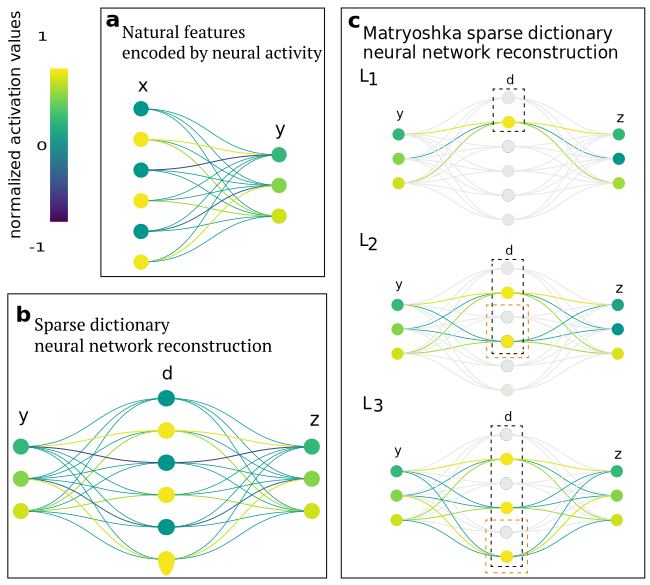
\includegraphics[width=\linewidth]{figures/sdnn_arch.pdf}
    \end{minipage}
    \begin{minipage}{0.37\linewidth}
    \caption{
        \textbf{MINI's sparse dictionary neural network architecture.} \\
        \small (\textbf{a}) Natural features $x$ get encoded by neural activity $y$. (\textbf{b}) A sparse dictionary neural network attempts to recreate neural activity $\hat{y}$ from $y$. If $\hat{y}$ tries to recreate $y$ exactly, then the model is an autoencoder, while in other situations it may be a transcoder or crosscoder. \textbf{c}) A Matryoshka spare dictionary neural network segments the latent space into multiple levels, each of which attempts to do a full reconstruction of the target neural activity. In this case, latents exclusive to the highest-level will often correspond to high-level features (e.g. a round object), while latents exclusive to the lowest-level will often correspond to low-level features (e.g. a basketball).
    }
    \label{fig:sdnn_arch}
    \end{minipage}
\end{figure}

\begin{itemize}
    \item Usefulness of SDL methods in Mech interp.
    
    \item Variant of MSAE as variant of SAE.
    \begin{itemize}
        \item Briefly mention other archs tried: batchTopK winner for sparsity enforcement.
    \end{itemize}
    
    \item In addition to MSAE levels width, briefly mention hyperparameters, expound in Appendix.
    \begin{itemize}
        \item topk per level, loss X per level, seq len for neural data, seq len for latent space used with transformer layer in decoder
    \end{itemize}
    
    \item Show latex formulas for encoder, decoder, total loss.
\end{itemize}
